% Chapter 6

\chapter{Evaluation}% Main chapter title

\label{Chapter6} % For referencing the chapter elsewhere, use \ref{Chapter6} 
To determine whether the propositions of the database model and the database application design in Chapter 4 and Chapter 5 meet the user requirements, four experiments are performed. The experiments are real-time data collecting, importing data from EDF file format, exporting data from the database to EDF file format, querying data from the database. In addition to the four experiments, a mixed of the experiments together with graphical visualization is also evaluated. When performing a database evaluation, the most important metrics under evaluating are the read/write speed and the size of the database. That is, time to retrieve data and space to store data must meet the user requirements. Moreover, the database application must ensure no data lost, or data corrupted when storing and retrieving. With respect to mobile platforms, which are usually limited resources and battery driven, the database application must also use the resources in an efficient way. Since a database connection is shared for many activities while the application is used, it needs to evaluate time each activity uses the connection.\\
The extensibility for future use is clearly presented in the design chapter, and therefore not be evaluated in this section. As discussed in the design chapter, the database design is a platform independent, it can easily be implemented on a bio-signals collector application such as CESAR acquisition tool to minimize the sending and receiving overhead between collectors and the database application server. There are some common experiments when evaluating a database design and database application. The evaluated experiments in this chapter, therefore, inspire applications which want to implement the database design.\\
The goals of the experiments are to evaluate the feasibility of the database model, and to convince the reader that the functional and non-functional requirements for the database modeling and the database application are satisfied by measuring performance of the read/write on the database, performance of the database application, and storage capacity. In this section, each experiment is evaluated with respect to reasons it is performed, workloads used, evaluated metrics, procedure to evaluate, and the results from the experiment.\\
A BITalino plugged kit, two Android devices, and a CESAR acquisition simulator run on macOS Sierra are using for the experiments. Table \ref{tab:DevicesSpecs} presents specifications for the used devices in this chapter.
\section{Real-time data collecting experiment}
\begin{table}
\begin{center}
\begin{tabular}{ |p{2cm}|p{2.7cm}|p{2.8cm}|p{3cm}|}
 \hline
 Technology&Xiaomi Mi5& MacBook Retina\newline 15 Late 2013&BITalino BT\newline plugged kit\\
 \hline
 OS&Android 7.0& macOS Sierra&n/a\\
 \hline
 RAM&3GB&16GB&n/a\\
 \hline
 CHIP&Snapdragon 820\newline 4 core 1.8GHz&Intel core i7\newline 4 core 2.3GHz&MCU with sampling rate 1, 10, 100, or 1000Hz\\
 \hline
 Wi-Fi&802.11\newline a/b/g/n/ac& 802.11\newline a/b/g/ac&n/a\\
 \hline
 Bluetooth&v4.2&v4.0&v2.0, range 10m\\
 \hline
 Battery&3000mAh&8440mAh&500mAh or 1500mAh\\
 \hline
\end{tabular}
\end{center}
\caption{Used devices specifications}
\label{tab:DevicesSpecs}
\end{table}
The database application is required to collect and store bio-signal data from CESAR acquisition tool to the designed database model on a mobile device. The CESAR acquisition tool sends data with four different frequencies, that are 1Hz, 10Hz, 100Hz, and 1000Hz. The goal of the acquisition tool is to collect OSA data, hence, a duration of the experiment can be more than 12 hours. The current version of CESAR acquisition tool cannot delivery samples at 1000Hz; the tool stops sending data after 30min-40min. Therefore, a CESAR acquisition simulator is used for sending samples with frequencies 1000Hz or higher. Goals of the experiment are to evaluate the robustness of the database application, database read/write performances, database size when collecting data from many different sources with different frequencies. Since the application is run on a mobile platform where the resources are limited, usage resources such as CPU and battery consumption are also evaluated in this section.
\subsection{Experiment workloads}
The database application collects samples from multiple sources simultaneously, in which each source sends data at different frequencies. A mount of samples the database need to store at a certain time is depended on the number of current connected sources and the number of channels that belong to each source. In addition, when the frequencies are high, the number of arriving samples in a period time becomes very large; it has a huge impact on the storing process of the database application. Since the application uses batch processing to manage and store incoming samples, a batch size highly influents the performance of the application. The batch size is defined by multiplying the buffer duration with arrival rate. Therefore, the workloads for the experiment are a buffer duration in second, an arrival rate of a source in Hz, a number of channels (total channels from the connected sources).
\subsection{Experiment metrics}
Evaluation metrics must highlight the goals and the workloads of the experiment. In the real-time data collecting experiment, the application has to parse arrival packages into relevant objects for the database. Therefore, percent CPU usage and power consumption are considered the metrics used in the evaluation. Percent CPU usage is obtained by using command “adb shell busybox top –d 5”. This command generates an output which contains the information about CPU usage for each application, and the output is printed in the standard output in each five seconds. The outputs from the command are redirected to a text file, and the file are used for making visualization. Listing \ref{listing:BUSYBOXTOP} presents a sample output from the command. As presented in the listing, the CPU usage of the application is 25.6\%. Power consumption can be obtained after a collecting process is finished by checking the battery usage in the Android system. Figure \ref{fig:Figures/PowerMetric} presents an example where the power consumption for each application is calcualted in percent of total power drained off.\\
\begin{figure}
    \centering
    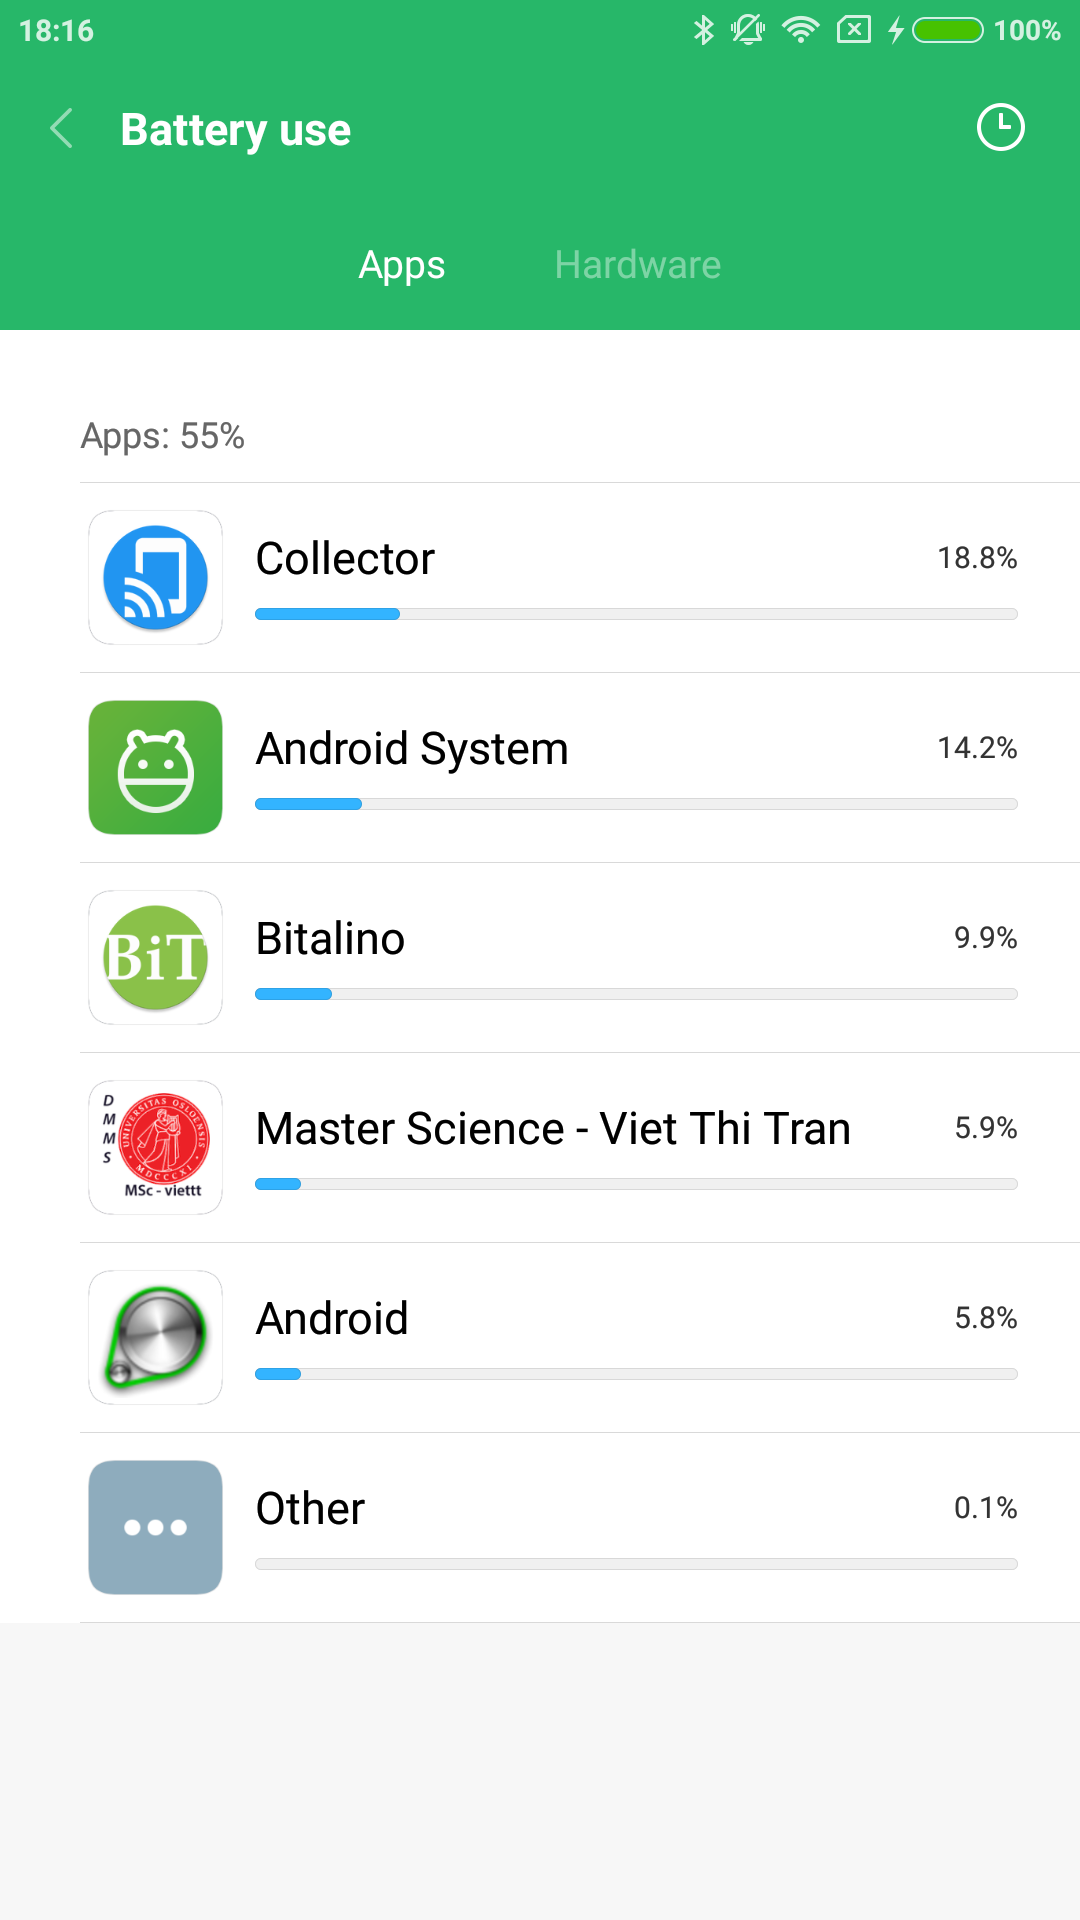
\includegraphics[width=0.4\textwidth]{Figures/PowerMetric.png}
    \caption{Battery usage}
    \label{fig:Figures/PowerMetric}
\end{figure}
Since the application uses batch processing to manage arrival data, when the temporary buffer is full, a SQLite transaction is requested for inserting data into the database. While the transaction is performed, it locks the entire database file. Hence, the SQLite usage time in millisecond for different batch size, and the number of insertions per millisecond are another metrics for the experiment. Nonetheless, the application is implemented on the mobile platform where resources are limited, it is good to see how big the database grows in megabytes for different workloads in a specific period time.
\subsection{Experiment setup and results}
\begin{minipage}{\linewidth}
\begin{lstlisting}[caption={A sample of five seconds fragment ouput from the command}, label = {listing:BUSYBOXTOP}, captionpos=b, basicstyle=\ttfamily\footnotesize]
viettt$  adb shell busybox top  d 5 > File1.txt

[H[JMem: 2720896K used, 39068K free, 0K shrd, 2496K buff, 537K cached
CPU: 27.2% usr  3.6% sys  0.0% nic 67.7% idle  0.2% io  0.6% irq  0.3% sirq
Load average: 6.89 6.25 5.88 3/2638 12713
[7m  PID  PPID USER     STAT   VSZ %VSZ CPU %CPU COMMAND[0m
11161   769 app_199  S <  2310m 85.3   0 25.6 {i.viettt.mscosa} no.uio.ifi.viett
  585     1 system   R <   133m  4.9   1  1.8 /system/bin/surfaceflinger
 1521   769 system   S    2530m 93.4   0  1.1 system_server
10096     2 root     SW       0  0.0   0  0.3 [kworker/u8:3]
  602     1 system   S    68152  2.4   2  0.3 /system/vendor/bin/mm-pp-dpps
12592     2 root     DW       0  0.0   0  0.3 [mdss_fb0]
  578     1 system   S     9424  0.3   0  0.3 /system/bin/servicemanager
10861     2 root     DW       0  0.0   0  0.3 [kworker/u8:5]
    7     2 root     SW       0  0.0   3  0.2 [rcu_preempt]
 2021   769 system   S <  2417m 89.2   2  0.1 {ndroid.systemui} com.android.syst
12706 23916 shell    R     1416  0.0   3  0.1 busybox top d 5
....................
\end{lstlisting}
\end{minipage}
As described above, there are two workload generators that are used in the experiment, they are the CESAR acquisition tool, and the CESAR acquisition simulator. In addition, a workload which is the buffer duration for the application can be adjusted before performing a collecting process. A workload that is monitored (its value is adjusted before a collecting process starts) is called the experimental workload. The other workloads that are unmonitored (their values must be keep the same for each collecting process) are called control workloads. Calculated results after each collecting process are called the responsive metrics.\\
\begin{table}
\centering
\begin{tabular}{|p{4cm}|p{2cm}|p{2cm}|p{2cm}|p{2cm}|}
\hline
\multicolumn{2}{|c|}{\multirow{2}{*}{\begin{tabular}[c]{@{}c@{}}Responsive metrics\\ for different battery used\end{tabular}}} & \multicolumn{3}{c|}{\begin{tabular}[c]{@{}c@{}}Experimental workload\\ Buffer duration\end{tabular}} \\ \cline{3-5} 
\multicolumn{2}{|l|}{} & 10 second & 20 second & 30 second \\ \hline
\begin{tabular}[c]{@{}l@{}}CPU usage\\ (percent)\end{tabular} & 10min & text1.txt & text2.txt & text3.txt \\ \hline
\multirow{2}{*}{\begin{tabular}[c]{@{}l@{}}Power consumption\\ (percent)\end{tabular}} & 500mAh &  &  &  \\ \cline{2-5} 
 & 1500mAh &  &  &  \\ \hline
\multirow{2}{*}{\begin{tabular}[c]{@{}l@{}}SQLite usage time\\ (millisecond)\end{tabular}} & 500mAh &  &  &  \\ \cline{2-5} 
 & 1500mAh &  &  &  \\ \hline
\multirow{2}{*}{\begin{tabular}[c]{@{}l@{}}Database file size\\ (Megabytes)\end{tabular}} & 500mAh &  &  &  \\ \cline{2-5} 
 & 1500mAh &  &  &  \\ \hline
\multirow{2}{*}{\begin{tabular}[c]{@{}l@{}}Avg. nr. insertion \\ per millisecond\end{tabular}} & 500mAh &  &  &  \\ \cline{2-5} 
 & 1500mAh &  &  &  \\ \hline
\end{tabular}
\caption{Buffer duration}
\label{tab:BufferDuration}
\end{table}
Table \ref{tab:BufferDuration} presents the responsive metrics for an experiment where the experimental workload is a buffer duration; control workloads are arrival rate and number of used channels. In this experiment, arrival rate is 100Hz, and all channels of the CESAR acquisition tool are used (6 channels). Likewise, in Table \ref{tab:ArrivalRate}, the experimental workload is arrival rate; control workloads are buffer duration (5 second), and all channels of the CESAR acquisition tool are used (6 channels). The number of channels is chosen as the experimental workload in Table \ref{tab:NrOfChannels}. In this case, the control workloads are the buffer duration (5s) and arrival rate (100Hz).\\
\begin{table}
\centering
\begin{tabular}{|p{3.5cm}|p{1.7cm}|p{1.7cm}|p{1.7cm}|p{1.7cm}|p{1.7cm}|}
\hline
\multicolumn{2}{|c|}{\multirow{2}{*}{\begin{tabular}[c]{@{}c@{}}Responsive metrics\\ for different battery used\end{tabular}}} & \multicolumn{4}{c|}{\begin{tabular}[c]{@{}c@{}}Experimental workload\\ Arrival rate\end{tabular}} \\ \cline{3-6} 
\multicolumn{2}{|l|}{} & 1Hz & 10Hz & 100Hz & 1000Hz \\ \hline
\begin{tabular}[c]{@{}l@{}}CPU usage\\ (percent)\end{tabular} & 10min & text1.txt & text2.txt & text3.txt & text4.txt \\ \hline
\multirow{2}{*}{\begin{tabular}[c]{@{}l@{}}Power consumption\\ (percent)\end{tabular}} & 500mAh &  &  &  &  \\ \cline{2-6} 
 & 1500mAh &  &  &  &  \\ \hline
\multirow{2}{*}{\begin{tabular}[c]{@{}l@{}}SQLite usage time\\ (millisecond)\end{tabular}} & 500mAh &  &  &  &  \\ \cline{2-6} 
 & 1500mAh &  &  &  &  \\ \hline
\multirow{2}{*}{\begin{tabular}[c]{@{}l@{}}Database file size\\ (Megabytes)\end{tabular}} & 500mAh &  &  &  &  \\ \cline{2-6} 
 & 1500mAh &  &  &  &  \\ \hline
\multirow{2}{*}{\begin{tabular}[c]{@{}l@{}}Avg. nr. insertion \\ per millisecond\end{tabular}} & 500mAh &  &  &  &  \\ \cline{2-6} 
 & 1500mAh &  &  &  &  \\ \hline
\end{tabular}
\caption{Arrival rate}
\label{tab:ArrivalRate}
\end{table}
For each experiment, a collecting process is iterated three times. The first collecting iteration is 10 minutes; it is because the workload parameters are not changed under the collecting process, hence it is no need to perform long time evaluation for the CPU usage. The BITalino can be powered by different battery capacities; a 700mAh and 1500mAh, which can offer about 5 to 15 hours for collecting data, are used in the experiment. The second and the third iterations are therefore running until the full charged batteries of the BITalino become empty. The metrics that are evaluated for these iterations are the power consumption, SQLite usage time, the writing speed (average insertion per millisecond), and the size of the database after the iterations.\\
\begin{table}
\centering
\begin{tabular}{|p{4cm}|p{2cm}|p{2cm}|p{2cm}|p{2cm}|}
\hline
\multicolumn{2}{|c|}{\multirow{2}{*}{\begin{tabular}[c]{@{}c@{}}Responsive metrics\\ for different battery used\end{tabular}}} & \multicolumn{3}{c|}{\begin{tabular}[c]{@{}c@{}}Experimental workload\\ Number of channels\end{tabular}} \\ \cline{3-5} 
\multicolumn{2}{|l|}{} & 3  & 6 & 12 \\ \hline
\begin{tabular}[c]{@{}l@{}}CPU usage\\ (percent)\end{tabular} & 10min & text1.txt & text2.txt & text3.txt \\ \hline
\multirow{2}{*}{\begin{tabular}[c]{@{}l@{}}Power consumption\\ (percent)\end{tabular}} & 500mAh &  &  &  \\ \cline{2-5} 
 & 1500mAh &  &  &  \\ \hline
\multirow{2}{*}{\begin{tabular}[c]{@{}l@{}}SQLite usage time\\ (millisecond)\end{tabular}} & 500mAh &  &  &  \\ \cline{2-5} 
 & 1500mAh &  &  &  \\ \hline
\multirow{2}{*}{\begin{tabular}[c]{@{}l@{}}Database file size\\ (Megabytes)\end{tabular}} & 500mAh &  &  &  \\ \cline{2-5} 
 & 1500mAh &  &  &  \\ \hline
\multirow{2}{*}{\begin{tabular}[c]{@{}l@{}}Avg. nr. insertion \\ per millisecond\end{tabular}} & 500mAh &  &  &  \\ \cline{2-5} 
 & 1500mAh &  &  &  \\ \hline
\end{tabular}
\caption{Number of channels}
\label{tab:NrOfChannels}
\end{table}
\subsection{Discussion}
<WHEN I HAVE THE RESULTS, I WILL WRITE THIS SUBSECTION: HOW TO PARSE CPU USAGE FILE, HOW TO PLOT DATA... THEN, AS PRESENTED IN FIGURE ...>
\section{EDF importing experiment}
The database model is designed in the way that opens for all bio-signals, and can store data from other database sources if the sources support EDF exporting. In other words, the data base application is required to import data from EDF and EDF+ file formats. Goals of the experiment are to evaluate database writing performance and usage resources such as CPU and battery consumption, especially, when the application reads files simultaneously.
\subsection{Experiment workloads}
The database application reads sample data from multiple files simultaneously. Ideally, each sample from the files is parsed to an object in memory, then inserted into the database. However, each INSERT statement in SQLite has its own transaction, and SQLite can only do a few dozen transactions per second. The samples are, therefore, grouped into a transaction before performing a SQLite insertion. The transaction locks entire database file when it performs inserting. Hence, if the sample group is too large, it can cause either memory problem, or poor performance since other transactions have to wait for it. Therefore, the workloads for the experiment are a size of the sample group and the number of file read.
\subsection{Experiment metrics}
Metrics that are chosen to highlight the goals and workload of the experiment are the percent CPU usage, the percent power consumption, the size of a EDF file in the database, total time the experiment holds the shared SQLite connection, and how many samples are inserted to the database for each hold-time. The percent CPU usage and the power consumption need to be evaluated since the application need to parse the samples in the EDF file format to objects that can be stored into the database. In addition, the number of samples are inserted for each hold-time can be used for evaluating the writing performance of the database.
\subsection{Experiment setup and results}
\begin{lstlisting}[caption={Convert mit2edf by using terminal}, label = {listing:MIT2EDF}, captionpos=b]
(no options)Terminal $mit2edf -r a01 
(options)Terminal $mit2edf -r a01 [-v -h -p] -o phy1.edf
\end{lstlisting}
To generate workloads for the experiment, a function from Physionet which named mit2edf is used for exporting bio-signal data from Physionet databases to EDF file format. As presented in the manual page of the function, mit2edf creates an EDF file that contains the same data as the input files which are in form of Waveform Database format (header and signal files). However, the function is included in WFDB software package from Physionet, the user must install the package first. There are three options when using the function which are printing a brief usage summary, choosing a name for the exported edf (the exported file has the same name as the imported record), and printing debugging output. Listing \ref{listing:MIT2EDF} presents how to use the function to convert a01 record to EDF file format without options and with options on a Linux/Unix terminal.
\begin{table}
\centering
\begin{tabular}{|l|l|l|l|l|}
\hline
\multicolumn{2}{|c|}{\multirow{2}{*}{\begin{tabular}[c]{@{}c@{}}Responsive metrics\end{tabular}}} & \multicolumn{3}{l|}{\begin{tabular}[c]{@{}c@{}}Experimental workload\\ Number of files simultaneously read\end{tabular}} \\ \cline{3-5} 
\multicolumn{2}{|l|}{} & 1 & 2 & 3 \\ \hline
\multicolumn{2}{|l|}{\begin{tabular}[c]{@{}l@{}}CPU usage\\ (percent)\end{tabular}} & text1.txt & text2.txt & text3.txt \\ \hline
\multicolumn{2}{|l|}{\multirow{2}{*}{\begin{tabular}[c]{@{}l@{}}Power consumption\\ (percent)\end{tabular}}} & \multirow{2}{*}{} & \multirow{2}{*}{} & \multirow{2}{*}{} \\
\multicolumn{2}{|l|}{} &  &  &  \\ \hline
\multicolumn{2}{|l|}{\begin{tabular}[c]{@{}l@{}}SQLite usage time\\ (millisecond)\end{tabular}} &  &  &  \\ \hline
\multicolumn{2}{|l|}{\multirow{2}{*}{\begin{tabular}[c]{@{}l@{}}Database file size\\ (Megabytes)\end{tabular}}} & \multirow{2}{*}{} & \multirow{2}{*}{} & \multirow{2}{*}{} \\
\multicolumn{2}{|l|}{} &  &  &  \\ \hline
\multicolumn{2}{|l|}{\multirow{2}{*}{\begin{tabular}[c]{@{}l@{}}Avg. nr. insertion \\ per millisecond\end{tabular}}} & \multirow{2}{*}{} & \multirow{2}{*}{} & \multirow{2}{*}{} \\
\multicolumn{2}{|l|}{} &  &  &  \\ \hline
\end{tabular}
\caption{Number of files simultaneously read}
\label{tab:NrOfSIMULTANEOUSELYREAD}
\end{table}
Workloads that are used for the experiment are a01.edf, a02.edf, and a03.edf files, which are generated from a01, a02, and a03 records from CinC2000 data sets. Since the implementation for the EDF-reader uses the same algorithm (batching processing) as real-time importing, there are two factors that influent the goals of the experiments. They are the number of simultaneously EDF files read, and the buffer size (batch size). Table \ref{tab:NrOfSIMULTANEOUSELYREAD} presents the results for the experiment where the experimental workload is the number of simultaneously EDF files read. In this experiment, the batch size is 50000 samples, and is kept the same for three iterations. Table \ref{tab:NrOfSAMPLESBATCH} presents the results for the experiment after three iterations with batch size 50000, 100000 and 150000 samples respectively. Since the number of file read is not the experimental workload in each iteration, the number of file read and the used files must be the same for each iteration. a01.edf is chosen as the control workload for the experiment.
\begin{table}
\centering
\begin{tabular}{|l|l|l|l|l|}
\hline
\multicolumn{2}{|l|}{\multirow{2}{*}{\begin{tabular}[c]{@{}c@{}}Responsive metrics\end{tabular}}} & \multicolumn{3}{l|}{\begin{tabular}[c]{@{}c@{}}Experimental workload\\ Number of samples in batch\end{tabular}} \\ \cline{3-5} 
\multicolumn{2}{|l|}{} & 50000 & 100000 & 150000 \\ \hline
\multicolumn{2}{|l|}{\begin{tabular}[c]{@{}l@{}}CPU usage\\ (percent)\end{tabular}} & text1.txt & text2.txt & text3.txt \\ \hline
\multicolumn{2}{|l|}{\multirow{2}{*}{\begin{tabular}[c]{@{}l@{}}Power consumption\\ (percent)\end{tabular}}} & \multirow{2}{*}{} & \multirow{2}{*}{} & \multirow{2}{*}{} \\
\multicolumn{2}{|l|}{} &  &  &  \\ \hline
\multicolumn{2}{|l|}{\begin{tabular}[c]{@{}l@{}}SQLite usage time\\ (millisecond)\end{tabular}} &  &  &  \\ \hline
\multicolumn{2}{|l|}{\multirow{2}{*}{\begin{tabular}[c]{@{}l@{}}Database file size\\ (Megabytes)\end{tabular}}} & \multirow{2}{*}{} & \multirow{2}{*}{} & \multirow{2}{*}{} \\
\multicolumn{2}{|l|}{} &  &  &  \\ \hline
\multicolumn{2}{|l|}{\multirow{2}{*}{\begin{tabular}[c]{@{}l@{}}Avg. nr. insertion \\ per millisecond\end{tabular}}} & \multirow{2}{*}{} & \multirow{2}{*}{} & \multirow{2}{*}{} \\
\multicolumn{2}{|l|}{} &  &  &  \\ \hline
\end{tabular}
\caption{Number of samples in batch}
\label{tab:NrOfSAMPLESBATCH}
\end{table}
\subsection{Discussion}
<WHEN I HAVE THE RESULTS, I WILL WRITE THIS SUBSECTION: HOW TO PLOT DATA... THEN, AS PRESENTED IN FIGURE ...>
\section{EDF exporting experiment}
The database application is required to export data to EDF file format for sharing or for backup data purposes. Since each record in the database is defined for a specific channel of a source (a.k.a channel record), and if records have the same patient id, physician id and timestamp, they are considered to be belonged to the same collecting process (a whole record). It is because a patient can use multiple sensor platforms to collect data. By choosing records with the same patient id, physician id and timestamp, a whole record can be retrieved. It is freely to choose which channel records to be included in the exported record; it is because sometimes a user needs data from some specific channels. EDF file format requires that a whole record need to be divided into small data records. A duration of the small data records is freely chosen. However, a data record size does not exceed 61440 bytes \citep{EDFpluss}. In the implementation of the database application, a data record is defined as a buffer in memory, and this buffer is flushed to the exported file when it is full. Hence, the data record size is also the buffer size which is defined by a summary of all channel buffer sizes. A channel buffer size is defined by multiplying the data record duration with the frequency of a channel.\\\\
$bufferSize=\sum_{i = 1}^{n}\frac{duration}{frequency\ channel(i)}$\\\\
Goals of the experiment are to evaluate the read performance of the database and resource usage such as percent CPU usage and battery consumption. In addition, time usage for exporting data is also evaluated in this subsection.
\subsection{Experiment workloads}
As presented in the high level design of the database application, the application continuously queries part of a record into a buffer, then writes the buffer to the exported EDF file. The application requests a database access for each selected record. Therefore, if the number of selected records for exporting is large, the application needs to access the database multiple times. In addition, although a large buffer may cause a memory problem if the memory of the used mobile device is small, it reduces the number database access of the application. In other word, a small buffer causes overhead for database accessing.
Therefore, experimental workloads for the experiment are the number of exporting records and the duration of a data record (a.k.a the buffer size).
\subsection{Experiment metrics}
A record can be very large, since it can be collected in long time. It takes time to export data, especially when a record is large, and a buffer size is small. In this case, the database application needs to query data multiple times to avoid memory corruption since the record cannot be kept in memory for exporting. Therefore, beside metrics such as CPU usage, power consumption, database read performance, and shared SQLite connect time usage as discussed in the experiments above, time it takes to export a record to EDF file format is also one of the chosen metrics in the experiment.
\subsection{Experiment setup and results}
Since the experimental workloads for the experiment are the number of exporting records and the duration of a data record, by changing values of the experimental workloads, the EDF exporting experiment can be evaluated by assessing the results of the experiment.\\
\begin{table}
\centering
\begin{tabular}{|l|l|l|l|l|}
\hline
\multicolumn{2}{|l|}{\multirow{2}{*}{\begin{tabular}[c]{@{}c@{}}Responsive metrics\end{tabular}}} & \multicolumn{3}{l|}{\begin{tabular}[c]{@{}c@{}}Experimental workload\\ Number of exporting records\end{tabular}} \\ \cline{3-5} 
\multicolumn{2}{|l|}{} & 5 & 10 & 15 \\ \hline
\multicolumn{2}{|l|}{\begin{tabular}[c]{@{}l@{}}CPU usage\\ (percent)\end{tabular}} & text1.txt & text2.txt & text3.txt \\ \hline
\multicolumn{2}{|l|}{\multirow{2}{*}{\begin{tabular}[c]{@{}l@{}}Power consumption\\ (percent)\end{tabular}}} & \multirow{2}{*}{} & \multirow{2}{*}{} & \multirow{2}{*}{} \\
\multicolumn{2}{|l|}{} &  &  &  \\ \hline
\multicolumn{2}{|l|}{\begin{tabular}[c]{@{}l@{}}SQLite usage time\\ (millisecond)\end{tabular}} &  &  &  \\ \hline
\multicolumn{2}{|l|}{\multirow{2}{*}{\begin{tabular}[c]{@{}l@{}}Exported file size\\ (Megabytes)\end{tabular}}} & \multirow{2}{*}{} & \multirow{2}{*}{} & \multirow{2}{*}{} \\
\multicolumn{2}{|l|}{} &  &  &  \\ \hline
\end{tabular}
\caption{Number of exporting records}
\label{tab:NrOfEXPORTINGRECORD}
\end{table}
Table \ref{tab:NrOfEXPORTINGRECORD} presents the results for the experiment where the experimental workload is the number of exporting record. The experiment is performed with 5, 10, and 15 records for each iteration. The data record duration that is used in each iteration is five seconds. Table \ref{tab:DURATIONOFDATAREOCRD}, on the other hand, presents the results for the experiment with different data record durations, which are one second, five seconds and ten seconds. The number of exporting records is 10, and is the same for each run in the experiment.\\
\begin{table}
\centering
\begin{tabular}{|l|l|l|l|l|}
\hline
\multicolumn{2}{|l|}{\multirow{2}{*}{\begin{tabular}[c]{@{}c@{}}Responsive metrics\end{tabular}}} & \multicolumn{3}{l|}{\begin{tabular}[c]{@{}c@{}}Experimental workload\\ Duration of a data record in EDF file\end{tabular}} \\ \cline{3-5} 
\multicolumn{2}{|l|}{} & 1s & 5s & 10s \\ \hline
\multicolumn{2}{|l|}{\begin{tabular}[c]{@{}l@{}}CPU usage\\ (percent)\end{tabular}} & text1.txt & text2.txt & text3.txt \\ \hline
\multicolumn{2}{|l|}{\multirow{2}{*}{\begin{tabular}[c]{@{}l@{}}Power consumption\\ (percent)\end{tabular}}} & \multirow{2}{*}{} & \multirow{2}{*}{} & \multirow{2}{*}{} \\
\multicolumn{2}{|l|}{} &  &  &  \\ \hline
\multicolumn{2}{|l|}{\begin{tabular}[c]{@{}l@{}}SQLite usage time\\ (millisecond)\end{tabular}} &  &  &  \\ \hline
\multicolumn{2}{|l|}{\multirow{2}{*}{\begin{tabular}[c]{@{}l@{}}Exported file size\\ (Megabytes)\end{tabular}}} & \multirow{2}{*}{} & \multirow{2}{*}{} & \multirow{2}{*}{} \\
\multicolumn{2}{|l|}{} &  &  &  \\ \hline
\end{tabular}
\caption{Duration of a data record in EDF file}
\label{tab:DURATIONOFDATAREOCRD}
\end{table}
\subsection{Discussion}
<WHEN I HAVE THE RESULTS, I WILL WRITE THIS SUBSECTION: HOW TO PLOT DATA... THEN, AS PRESENTED IN FIGURE ...>
\section{Querying data experiment}
When processing a SQL query, a database management system (DBMS) goes through at least three steps. The first step is to parse SQL query into a data structure that can be processed by the DBMS. In this step, the syntax and semantic of the query are checked to determine if the SQL statement is syntactic validity, and if the statement is meaningful, i.e. whether the columns and tables are existed in the database. The second step is to optimize the query. That is, by using a set of equivalence rules, the query optimizer can generate many equivalent plans in which a cost is assigned for each plan. The plan that has a lowest cost is taken to the third step which is to execute the query plan. Although the SQL query is optimized before querying, the complexity of the SQL query and the results from the query are not changed.\\
Goals of the experiment is to evaluate the resource usage and performance of the database application with respect to the complexity of the queries, and the size of the results.
\subsection{Experiment workloads}
In SQLite, all queries are simple select statement. A simple select statement is often processed via four steps \citep{SQLITE_SELECT}.
\begin{itemize}
\item From clause processing: The input data of the statement are specified in this step.
\item Where clause processing: The expression in the clause helps to filter the return data.
\item Group by, having processing: groups of data are calculating and aggregating with respect to the filter expression in having.
\item Distinct / ALL keyword processing: result rows are return (duplicate rows are removed if “distinct” is specified).
\end{itemize}
A compound query statement is defined via connecting multiple simple select statement by using UNION, UNION ALL, etc.\\
Workloads for the experiment are therefore depended on the FROM clause, and whether statements are compound statements. As presented in SQLite \citep{SQLITE_SELECT}, all join-operators are based on Cartesian product of the left hand side (N rows) and right hand side (M rows) of the datasets. The results from the join are therefore NxM rows. In other words, the complexity when joining two table is O(MxN). The complexity is increased by the number of tables that are stated in the FROM clause. Moreover, if the result from the query is too large to hold in the memory, the DBMS musts pass the database multiple times (multiple-passes).\\
\begin{table}
\centering
\begin{tabular}{|l|c|c|}
\hline
Table & Number of columns & Approximate records \\ \hline
SensorSource & 3 & \textless100 \\ \hline
Patient & 7 & \textless100 \\ \hline
Physician & 4 & \textless100 \\ \hline
Clinic & 5 & \textless100 \\ \hline
Person & 8 & \textless100 \\ \hline
Channel & 11 & \textless1000 \\ \hline
Record & 10 & \textless1000 \\ \hline
RecordAnnotation & 2 & \textless1000 \\ \hline
Annotation & 5 & \textless1000 \\ \hline
Sample & 3 & \textgreater 1 million \\ \hline
\end{tabular}
\caption{Datasets in the database}
\label{tab:dataSETs}
\end{table}
As presented in Table \ref{tab:dataSETs}, the heaviest table is the Sample table, and together with the complexity of queries, they are therefore considered the main workloads of the experiment. There are four queries that are used for evaluating the experiment; the queries are described as follow:
\begin{itemize}
\item \textbf{Query 1:} A relatively small dataset is scanned (a.k.a simple query with small result). Any tables presented in Table \ref{tab:dataSETs}, as long as not the table Sample, can be chosen for this query.
\item \textbf{Query 2:} A relatively large dataset is scanned (a.k.a simple query with large result). 
\item \textbf{Query 3:} All presented tables in Table \ref{tab:dataSETs} are joined, then an aggregate function, i.e. count, sum, max, etc., is applied to have a small result (a.k.a complex query with small result).
\item \textbf{Query 4:} All presented tables in Table \ref{tab:dataSETs} are joined, no filters are applied in this query (a.k.a complex query with large result).
\end{itemize}
\subsection{Experiment metrics}
Metrics that are used for evaluating the experiment must highlight the resource usage and performance of the database application when executing different queries with different complexity. Therefore, the metrics that are chosen for the experiment are percent CPU usage, power consumption, and response time for queries. 
\subsection{Experiment setup and results}
\begin{table}
\centering
\begin{tabular}{|c|l|c|c|c|c|}
\hline
\multicolumn{1}{|l|}{\multirow{2}{*}{\begin{tabular}[c]{@{}l@{}}Query\\ Number\end{tabular}}} & \multicolumn{1}{c|}{\multirow{2}{*}{Table(s)}} & \multicolumn{2}{c|}{Input size} & \multicolumn{2}{c|}{Output size} \\ \cline{3-6} 
\multicolumn{1}{|l|}{} & \multicolumn{1}{c|}{} & MB & \# records & MB & \# records \\ \hline
1 & Channel &  &  &  &  \\ \hline
2 & Sample &  &  &  &  \\ \hline
3 & All tables &  &  &  &  \\ \hline
4 & All tables &  &  &  &  \\ \hline
\end{tabular}
\caption{Query statistics for the queries}
\label{tab:QUERYSTATISTICS}
\end{table}
The described queries in the subsection workload of this experiment are translated into SQLite code as follow:
\begin{itemize}
\item \textbf{Query 1:} The whole table Channel is chosen to be scanned.\\\texttt{select * from Channel}
\item \textbf{Query 2:} Since the table Sample is the largest, it is chosen for this query.\\
\texttt{select * from Sample}
\item \textbf{Query 3:} This query counts number of rows return from Cartesian product all tables.\\
\texttt{select count(*) from SensorSource, Patient, Physician, Clinic, Person, Channel, Record, RecordAnnotation, Annotation, Sample}
\item \textbf{Query 4:} This query return all rows from Cartesian product all tables.\\
\texttt{select * from SensorSource, Patient, Physician, Clinic, Person, Channel, Record, RecordAnnotation, Annotation, Sample}
\end{itemize}
Table \ref{tab:QUERYSTATISTICS} presents query statistics after executing the queries, while Table \ref{tab:QUERYING} presents the results for the experiment.
\begin{table}
\centering
\begin{tabular}{|l|l|c|c|c|c|}
\hline
\multicolumn{2}{|c|}{\multirow{2}{*}{\begin{tabular}[c]{@{}c@{}}Responsive metrics\end{tabular}}} & \multicolumn{4}{c|}{\begin{tabular}[c]{@{}c@{}}Experimental workload\end{tabular}} \\ \cline{3-6} 
\multicolumn{2}{|c|}{} & \multicolumn{1}{l|}{\begin{tabular}[c]{@{}l@{}}Simple query-\\ small result\end{tabular}} & \multicolumn{1}{l|}{\begin{tabular}[c]{@{}l@{}}Simple query-\\ large result\end{tabular}} & \multicolumn{1}{l|}{\begin{tabular}[c]{@{}l@{}}Complex query-\\ small result\end{tabular}} & \multicolumn{1}{l|}{\begin{tabular}[c]{@{}l@{}}Complex query-\\ small result\end{tabular}} \\ \hline
\multicolumn{2}{|l|}{\begin{tabular}[c]{@{}l@{}}CPU usage\\ (percent)\end{tabular}} & text1.txt & text2.txt & text3.txt & text4.txt \\ \hline
\multicolumn{2}{|l|}{\multirow{2}{*}{\begin{tabular}[c]{@{}l@{}}Power consumption\\ (percent)\end{tabular}}} & \multirow{2}{*}{} & \multirow{2}{*}{} & \multirow{2}{*}{} & \multirow{2}{*}{} \\
\multicolumn{2}{|l|}{} &  &  &  &  \\ \hline
\multicolumn{2}{|l|}{\begin{tabular}[c]{@{}l@{}}Executing ime\\ (millisecond)\end{tabular}} &  &  &  &  \\ \hline
\end{tabular}
\caption{Executing time and resource usage for the queries}
\label{tab:QUERYING}
\end{table}
\subsection{Discussion}
<WHEN I HAVE THE RESULTS, I WILL WRITE THIS SUBSECTION: HOW TO PLOT DATA... THEN, AS PRESENTED IN FIGURE ...>
\section{Stress test with visualization and mixed tasks experiment}
It is possible that a user collects data from multiple sensor sources to the database, and plots the collected data on a graphical view while there is an exporting process is running. In other words, the application usually performs multiple tasks simultaneously rather than finishes a task before beginning the others.\\
Therefore, goals of the experiment are to evaluate database read/write performances, database size when collecting data from many different sources (both EDF files and CESAR acquisition tool), and resource usage such as CPU and battery consumption.
\subsection{Experiment workloads and metrics}
Workloads for this experiment are borrowed from the experiments above, which are buffer duration, arrival rate, number of collecting channel (these workloads come from the real-time experiment), number of file simultaneously read, number of sample in a batch (these workloads are from EDF importing experiment), number of exporting records, duration of a data record in the exported EDF file (from the EDF exporting experiment), and the complexity of queries a user want to execute.\\
Metrics that are chosen in this experiment must highlighting the database application performance, the size of the database, and resource usage. Therefore, percent CPU usage, power consumption, database size in megabytes, and SQLite time usage in millisecond for each task are chosen as metrics for the evaluation.
\subsection{Experiment setup and results}
Each experiment, which is presented the previous sections, is evaluated with three different workloads. These workloads are increased after each run. Workloads for this experiment are combined of the workloads for each iteration of the experiments. The workloads are used for three iterations (three run) respectively in both real-time and non-real-time visualizations. However, the experiment is not performed in six or twelve hours as in the real-time experiment, it is finished as long as the files are read and/or exported. The querying experiment is not included in this experiment. It is because an executing of a query is very fast compared with reading or writing process, and to repeat the same query to keep synchronization with reading or writing process in order to evaluate the experiment is not a good idea since the DBMS caches the result of the query.
\subsection{Discussion}
<WHEN I HAVE THE RESULTS, I WILL WRITE THIS SUBSECTION: HOW TO PLOT DATA... THEN, AS PRESENTED IN FIGURE ...>
\begin{table}
\centering
\begin{tabular}{|l|c|c|c|}
\hline
\multicolumn{1}{|c|}{\multirow{2}{*}{\begin{tabular}[c]{@{}c@{}}Workloads\\ (real-time plotting)\end{tabular}}} & \multicolumn{3}{c|}{Responsive metrics} \\ \cline{2-4} 
\multicolumn{1}{|c|}{} & \begin{tabular}[c]{@{}c@{}}CPU usage \\ (percent)\end{tabular} & \begin{tabular}[c]{@{}c@{}}Power consumption \\ (percent)\end{tabular} & \begin{tabular}[c]{@{}c@{}}Database size \\ (Megabytes)\end{tabular} \\ \hline
\begin{tabular}[c]{@{}l@{}}Buffer duration: 5s\\ Arrival rate: 1Hz\\ Nr. channel: 3\\ File read: 1\\ Batch size: 50k\\ Nr. exporting record: 5\\ Data record duration: 1s\end{tabular} &  &  &  \\ \hline
\begin{tabular}[c]{@{}l@{}}Buffer duration: 10s\\ Arrival rate: 10Hz\\ Nr. channel: 6\\ File read: 2\\ Batch size: 100k\\ Nr. exporting record: 10\\ Data record duration: 5s\end{tabular} &  &  &  \\ \hline
\begin{tabular}[c]{@{}l@{}}Buffer duration: 15s\\ Arrival rate: 100Hz\\ Nr. channel: 12\\ File read: 3\\ Batch size: 150k\\ Nr. exporting record: 15\\ Data record duration: 10s\end{tabular} &  &  &  \\ \hline
\end{tabular}
\caption{Mixed tasks with real-time visualization}
\label{concept2}
\end{table}
\begin{table}
\centering
\begin{tabular}{|l|c|c|c|}
\hline
\multicolumn{1}{|c|}{\multirow{2}{*}{\begin{tabular}[c]{@{}c@{}}Workloads\\ (with plotting data \\ from the database)\end{tabular}}} & \multicolumn{3}{c|}{Responsive metrics} \\ \cline{2-4} 
\multicolumn{1}{|c|}{} & \begin{tabular}[c]{@{}c@{}}CPU usage \\ (percent)\end{tabular} & \begin{tabular}[c]{@{}c@{}}Power consumption \\ (percent)\end{tabular} & \begin{tabular}[c]{@{}c@{}}Database size \\ (Megabytes)\end{tabular} \\ \hline
\begin{tabular}[c]{@{}l@{}}Buffer duration: 5s\\ Arrival rate: 1Hz\\ Nr. channel: 3\\ File read: 1\\ Batch size: 50k\\ Nr. exporting record: 5\\ Data record duration: 1s\end{tabular} &  &  &  \\ \hline
\begin{tabular}[c]{@{}l@{}}Buffer duration: 10s\\ Arrival rate: 10Hz\\ Nr. channel: 6\\ File read: 2\\ Batch size: 100k\\ Nr. exporting record: 10\\ Data record duration: 5s\end{tabular} &  &  &  \\ \hline
\begin{tabular}[c]{@{}l@{}}Buffer duration: 15s\\ Arrival rate: 100Hz\\ Nr. channel: 12\\ File read: 3\\ Batch size: 150k\\ Nr. exporting record: 15\\ Data record duration: 10s\end{tabular} &  &  &  \\ \hline
\end{tabular}
\caption{Mixed tasks with visualization data from the database}
\label{concept3}
\end{table}